% !TEX program = pdflatex
\RequirePackage[l2tabu, orthodox]{nag}
\documentclass{article}

% FONTS
\usepackage[T1]{fontenc}

% Replace default Latin Modern typewriter with its proportional counterpart
% http://www.tug.dk/FontCatalogue/lmoderntypewriterprop/
\renewcommand*\ttdefault{lmvtt}


%%% OPTION 1 - Fourier Math + New Century Schoolbook + ParaType Sans

% % Import Fourier Math (this imposes its own New Century Schoolbook type)
% % http://www.ctan.org/tex-archive/fonts/fouriernc/
%\usepackage{fouriernc}
%\usepackage{amsmath}
% % Replace with TeX Gyre Schola version of New Century Schoolbook (must scale!)
% % http://www.tug.dk/FontCatalogue/tgschola/
%\usepackage[scale=0.92]{tgschola}
%\usepackage[scaled=0.88]{PTSans}

%% OPTION 2 - MathDesign Math + Bitstream Charter + ParaType Sans

% Import MathDesign (this brings along Bitstream Charter)
% http://www.ctan.org/tex-archive/fonts/mathdesign/
\usepackage[bitstream-charter]{mathdesign}
\usepackage{amsmath}
\usepackage[scaled=0.92]{PTSans}


% %%% OPTION 3 - MTPRO 2 Math + Termes Times + ParaType Sans

% \usepackage{tgtermes}
% \usepackage{amsmath}
% \usepackage[subscriptcorrection,
%             amssymbols,
%             mtpbb,
%             mtpcal,
%             nofontinfo  % suppresses all warnings
%            ]{mtpro2}
% \usepackage{scalefnt,letltxmacro}
% \LetLtxMacro{\oldtextsc}{\textsc}
% \renewcommand{\textsc}[1]{\oldtextsc{\scalefont{1.10}#1}}
% \usepackage[scaled=0.92]{PTSans}

% GEOMETRY
\usepackage[
  paper  = letterpaper,
  left   = 1.65in,
  right  = 1.65in,
  top    = 1.0in,
  bottom = 1.0in,
  ]{geometry}

% COLOR
\usepackage[usenames,dvipsnames]{xcolor}
\definecolor{shadecolor}{gray}{0.9}

% SPACING and TEXT
\usepackage[final,expansion=alltext]{microtype}
\usepackage[english]{babel}
\usepackage[parfill]{parskip}
\usepackage{afterpage}
\usepackage{framed}
\usepackage{verbatim}

%redefine the leftbar environment to accept a width and coloring options
\renewenvironment{leftbar}[1][\hsize]
{%
  \def\FrameCommand
  {%
    {\color{Gray}\vrule width 3pt}%
    \hspace{10pt}%
    %\hspace{0pt}\fboxsep=\FrameSep\colorbox{black!10}%
  }%
  \MakeFramed{\hsize#1\advance\hsize-\width\FrameRestore}%
}%
{\endMakeFramed}

% define a paragraph header function
\DeclareRobustCommand{\parhead}[1]{\textbf{#1}~}

% EDITING
% line numbering in left margin
\usepackage{lineno}
\renewcommand\linenumberfont{\normalfont
                             \footnotesize
                             \sffamily
                             \color{SkyBlue}}
% ragged paragraphs in right margin
\usepackage{ragged2e}
\DeclareRobustCommand{\sidenote}[1]{\marginpar{
                                    \RaggedRight
                                    \textcolor{Plum}{\textsf{#1}}}}
% paragraph counter in right margin
\newcommand{\parnum}{\bfseries\P\arabic{parcount}}
\newcounter{parcount}
\newcommand\p{%
    \stepcounter{parcount}%
    \leavevmode\marginpar[\hfill\parnum]{\parnum}%
}
% paragraph helper
%\DeclareRobustCommand{\PP}{\textcolor{Plum}{\P} }

% COUNTERS
\renewcommand{\labelenumi}{\color{black!67}{\arabic{enumi}.}}
\renewcommand{\labelenumii}{{\color{black!67}(\alph{enumii})}}
\renewcommand{\labelitemi}{{\color{black!67}\textbullet}}

% FIGURES
\usepackage{graphicx}
\usepackage[labelfont=bf]{caption}
\usepackage[format=hang]{subcaption}

% TABLES
\usepackage{booktabs}

% ALGORITHMS
\usepackage[algoruled]{algorithm2e}
\usepackage{listings}
\usepackage{fancyvrb}
\fvset{fontsize=\normalsize}

% BIBLIOGRAPHY
\usepackage{natbib}

% HYPERREF
\usepackage[colorlinks,linktoc=all]{hyperref}
\usepackage[all]{hypcap}
\hypersetup{citecolor=MidnightBlue}
\hypersetup{linkcolor=MidnightBlue}
\hypersetup{urlcolor=MidnightBlue}

% CLEVEREF must come after HYPERREF
\usepackage[nameinlink]{cleveref}

% ACRONYMS
\usepackage[acronym,smallcaps,nowarn]{glossaries}
% \makeglossaries

% COLOR DEFINITIONS
\newcommand{\red}[1]{\textcolor{BrickRed}{#1}}
\newcommand{\orange}[1]{\textcolor{BurntOrange}{#1}}
\newcommand{\green}[1]{\textcolor{OliveGreen}{#1}}
\newcommand{\blue}[1]{\textcolor{MidnightBlue}{#1}}
\newcommand{\gray}[1]{\textcolor{black!60}{#1}}

% LISTINGS DEFINTIONS
\lstdefinestyle{mystyle}{
    commentstyle=\color{OliveGreen},
    keywordstyle=\color{BurntOrange},
    numberstyle=\tiny\color{black!60},
    stringstyle=\color{MidnightBlue},
    basicstyle=\ttfamily,
    breakatwhitespace=false,
    breaklines=true,
    captionpos=b,
    keepspaces=true,
    numbers=left,
    numbersep=5pt,
    showspaces=false,
    showstringspaces=false,
    showtabs=false,
    tabsize=2
}
\lstset{style=mystyle}

\usepackage[colorinlistoftodos,
            prependcaption,
            textsize=tiny,
            backgroundcolor=yellow,
            linecolor=lightgray,
            bordercolor=lightgray]{todonotes}
\DeclareRobustCommand{\mb}[1]{\ensuremath{\boldsymbol{\mathbf{#1}}}}
\DeclareRobustCommand{\KL}[2]{\ensuremath{\textrm{KL}\left(#1\;\|\;#2\right)}}

\newcommand{\supp}{\textrm{supp}}

\newcommand{\E}{\mathbb{E}}
\newcommand{\Var}{\mathbb{V}\textrm{ar}}

% Redundant with reals, naturals, below
\newcommand{\bbN}{\mathbb{N}}
\newcommand{\bbZ}{\mathbb{Z}}
\newcommand{\bbR}{\mathbb{R}}
\newcommand{\bbS}{\mathbb{S}}


\newcommand{\bA}{\boldsymbol{A}}
\newcommand{\bB}{\boldsymbol{B}}
\newcommand{\bC}{\boldsymbol{C}}
\newcommand{\bD}{\boldsymbol{D}}
\newcommand{\bE}{\boldsymbol{E}}
\newcommand{\bF}{\boldsymbol{F}}
\newcommand{\bG}{\boldsymbol{G}}
\newcommand{\bH}{\boldsymbol{H}}
\newcommand{\bI}{\boldsymbol{I}}
\newcommand{\bJ}{\boldsymbol{J}}
\newcommand{\bK}{\boldsymbol{K}}
\newcommand{\bL}{\boldsymbol{L}}
\newcommand{\bM}{\boldsymbol{M}}
\newcommand{\bN}{\boldsymbol{N}}
\newcommand{\bO}{\boldsymbol{O}}
\newcommand{\bP}{\boldsymbol{P}}
\newcommand{\bQ}{\boldsymbol{Q}}
\newcommand{\bR}{\boldsymbol{R}}
\newcommand{\bS}{\boldsymbol{S}}
\newcommand{\bT}{\boldsymbol{T}}
\newcommand{\bU}{\boldsymbol{U}}
\newcommand{\bV}{\boldsymbol{V}}
\newcommand{\bW}{\boldsymbol{W}}
\newcommand{\bX}{\boldsymbol{X}}
\newcommand{\bY}{\boldsymbol{Y}}
\newcommand{\bZ}{\boldsymbol{Z}}
\newcommand{\ba}{\boldsymbol{a}}
\newcommand{\bb}{\boldsymbol{b}}
\newcommand{\bc}{\boldsymbol{c}}
\newcommand{\bd}{\boldsymbol{d}}
\newcommand{\be}{\boldsymbol{e}}
\newcommand{\bbf}{\boldsymbol{f}}
\newcommand{\bg}{\boldsymbol{g}}
\newcommand{\bh}{\boldsymbol{h}}
\newcommand{\bi}{\boldsymbol{i}}
\newcommand{\bj}{\boldsymbol{j}}
\newcommand{\bk}{\boldsymbol{k}}
\newcommand{\bl}{\boldsymbol{l}}
\newcommand{\bbm}{\boldsymbol{m}}
\newcommand{\bn}{\boldsymbol{n}}
\newcommand{\bo}{\boldsymbol{o}}
\newcommand{\bp}{\boldsymbol{p}}
\newcommand{\bq}{\boldsymbol{q}}
\newcommand{\br}{\boldsymbol{r}}
\newcommand{\bs}{\boldsymbol{s}}
\newcommand{\bt}{\boldsymbol{t}}
\newcommand{\bu}{\boldsymbol{u}}
\newcommand{\bv}{\boldsymbol{v}}
\newcommand{\bw}{\boldsymbol{w}}
\newcommand{\bx}{\boldsymbol{x}}
\newcommand{\by}{\boldsymbol{y}}
\newcommand{\bz}{\boldsymbol{z}}

\newcommand{\balpha}{\boldsymbol{\alpha}}
\newcommand{\bbeta}{\boldsymbol{\beta}}
\newcommand{\boldeta}{\boldsymbol{\eta}}
\newcommand{\bkappa}{\boldsymbol{\kappa}}
\newcommand{\bgamma}{\boldsymbol{\gamma}}
\newcommand{\blambda}{\boldsymbol{\lambda}}
\newcommand{\bmu}{\boldsymbol{\mu}}
\newcommand{\bnu}{\boldsymbol{\nu}}
\newcommand{\brho}{\boldsymbol{\rho}}
\newcommand{\bphi}{\boldsymbol{\phi}}
\newcommand{\bpi}{\boldsymbol{\pi}}
\newcommand{\bpsi}{\boldsymbol{\psi}}
\newcommand{\bsigma}{\boldsymbol{\sigma}}
\newcommand{\btheta}{\boldsymbol{\theta}}
\newcommand{\bomega}{\boldsymbol{\omega}}
\newcommand{\bxi}{\boldsymbol{\xi}}
\newcommand{\bGamma}{\boldsymbol{\Gamma}}
\newcommand{\bLambda}{\boldsymbol{\Lambda}}
\newcommand{\bOmega}{\boldsymbol{\Omega}}
\newcommand{\bPhi}{\boldsymbol{\Phi}}
\newcommand{\bPi}{\boldsymbol{\Pi}}
\newcommand{\bPsi}{\boldsymbol{\Psi}}
\newcommand{\bSigma}{\boldsymbol{\Sigma}}
\newcommand{\bTheta}{\boldsymbol{\Theta}}
\newcommand{\bUpsilon}{\boldsymbol{\Upsilon}}
\newcommand{\bXi}{\boldsymbol{\Xi}}
\newcommand{\bepsilon}{\boldsymbol{\epsilon}}

\newcommand{\mcA}{\mathcal{A}}
\newcommand{\mcB}{\mathcal{B}}
\newcommand{\mcC}{\mathcal{C}}
\newcommand{\mcD}{\mathcal{D}}
\newcommand{\mcE}{\mathcal{E}}
\newcommand{\mcF}{\mathcal{F}}
\newcommand{\mcG}{\mathcal{G}}
\newcommand{\mcH}{\mathcal{H}}
\newcommand{\mcI}{\mathcal{I}}
\newcommand{\mcJ}{\mathcal{J}}
\newcommand{\mcK}{\mathcal{K}}
\newcommand{\mcL}{\mathcal{L}}
\newcommand{\mcM}{\mathcal{M}}
\newcommand{\mcN}{\mathcal{N}}
\newcommand{\mcO}{\mathcal{O}}
\newcommand{\mcP}{\mathcal{P}}
\newcommand{\mcQ}{\mathcal{Q}}
\newcommand{\mcR}{\mathcal{R}}
\newcommand{\mcS}{\mathcal{S}}
\newcommand{\mcT}{\mathcal{T}}
\newcommand{\mcU}{\mathcal{U}}
\newcommand{\mcV}{\mathcal{V}}
\newcommand{\mcW}{\mathcal{W}}
\newcommand{\mcX}{\mathcal{X}}
\newcommand{\mcY}{\mathcal{Y}}
\newcommand{\mcZ}{\mathcal{Z}}

\newcommand{\trans}{\mathsf{T}}
\newcommand{\naturals}{\mathbb{N}}
\newcommand{\reals}{\mathbb{R}}
\def\argmax{\operatornamewithlimits{arg\,max}}
\def\argmin{\operatornamewithlimits{arg\,min}}

\newcommand{\distNormal}{\mathcal{N}}
\newcommand{\distGamma}{\mathrm{Gamma}}
\newcommand{\distBernoulli}{\mathrm{Bern}}
\newcommand{\distBinomial}{\mathrm{Bin}}
\newcommand{\distCategorical}{\mathrm{Cat}}
\newcommand{\distDirichlet}{\mathrm{Dir}}
\newcommand{\distMultinomial}{\mathrm{Mult}}
\newcommand{\distPolyaGamma}{\mathrm{PG}}
\newcommand{\distMNIW}{\mathrm{MNIW}}
\newcommand{\distBeta}{\mathrm{Beta}}

\newcommand{\prt}[1]{\frac{\partial}{\partial #1}}
\newcommand{\deriv}[1]{\frac{\mathrm{d}}{\mathrm{d} #1}}


\newcommand{\TODO}[1]{\textcolor{red}{[TODO: #1]}}

\newcommand{\bbI}{\mathbb{I}}
\newcommand{\bbE}{\mathbb{E}}
\newcommand{\bone}{\boldsymbol{1}}
\newcommand{\bigO}{\mathcal{O}}
\newcommand{\iid}[1]{\stackrel{\text{iid}}{#1}}
\newcommand\indep{\protect\mathpalette{\protect\independenT}{\perp}}
\def\independenT#1#2{\mathrel{\rlap{$#1#2$}\mkern4mu{#1#2}}}
\DeclareMathOperator{\Skew}{Skew}
\DeclareMathOperator{\Symm}{Sym}
\DeclareMathOperator{\tr}{tr}

%\DeclareMathOperator{\KL}{KL}
\newcommand{\given}{\, | \,}

\DeclareMathOperator{\diag}{diag}
\let\vec\relax% Set equal to \relax so that LaTeX thinks it's not defined
\DeclareMathOperator{\vec}{vec}
\let\Re\relax
\DeclareMathOperator{\Re}{\textup{Re}}
\let\Im\relax
\DeclareMathOperator{\Im}{\textup{Im}}

% Backcompat: dif and diff both work
\newcommand*\dif{\mathop{}\!\mathrm{d}}
\newcommand*\diff{\mathop{}\!\mathrm{d}}



% \linenumbers

\title{A Discussion of ``Nonparametric Bayes Modeling of Populations of Networks''\\
by Durante, Dunson, and Vogelstein}
\author{
  Scott W. Linderman and David M. Blei\\
  Columbia University
}
\date{\today}

\begin{document}
\maketitle

%\begin{abstract}
%\end{abstract}

\section{Introduction}

We congratulate the authors on their excellent paper.  While the
modeling of \emph{single} networks has received much attention, we agree
with the authors that the modeling of \emph{populations} of
networks has been largely overlooked.  Given that such data are
increasingly common in fields such as neuroscience, this paper makes a
timely contribution.  In this discussion, we consider a factorial
generalization of the proposed mixture of latent space models,
and we suggest cases in which factorial
models may naturally capture our intuition about the
underlying generative process of the data. We compare these two models using the
human brain data studied in the main paper, and we suggest some
avenues for future work.  Code to reproduce the figures in this
discussion is available
at~\url{https://github.com/blei-lab/factorial-network-models}.

\section{Model}
\citet{durante2016nonparametric}
propose a probabilistic model for populations of networks, which may
be represented as collections of binary adjacency matrices.
Let~$\{\bA_n\}_{n=1}^N$ denote such a collection, with
each~${A_n \in \{0,1\}^{V \times V}}$ representing the observed
connectivity of the~$n$-th network.  Entry~${A_{n,[u,v]}}$ is equal to
one edge if an edge is observed from vertex~$u$ to vertex~$v$ in
network~$n$, otherwise it is set to zero.  We assume the~$V$ vertices
are the same in all~$N$ networks.  Moreover, the networks are
undirected~(${A_{n,[u,v]} \equiv A_{n,[v,u]}}$) and without
self-loops~(${A_{n,[v,v]} \equiv 0}$). Thus, it suffices to model only
the lower triangular entries.

The authors build on the latent space model (LSM), a canonical model
in probabilistic network analysis \citep{hoff2002latent,
  hoff2008modeling}. An LSM is defined by the following parameters and
latent variables: a bias~${z_{u,v} \in \reals}$ for each edge; an
embedding~${\bx_v \in \reals^D}$ for each vertex; and a
positive-definite ``scaling''
matrix~${\bLambda = \diag(\blambda)}$,~$\blambda \in \reals_+^D$, that
determines the relative importance of the~$D$ latent dimensions.  For
convenience, let~${\bZ = \{\{z_{u,v}\}_{u=1}^V\}_{v=1}^{u-1}}$ denote
the set of per-connection biases.  Given these parameters and latent
variables, the edges are conditionally independent Bernoulli random
variables, and the likelihood of a network is,
\begin{align}
  p(\bA_{n} \given \bZ, \{\bx_v\}_{v=1}^V, \bLambda)
  &= \prod_{u=1}^V \prod_{v=1}^{u-1} \distBernoulli \left(A_{n, [u,v]} \given
    \sigma(z_{u,v} + \bx_u^\trans \bLambda \bx_v)\right),
\end{align}
where~${\distBernoulli(y \given \rho) = \rho^y (1-\rho)^{1-y}}$ is the Bernoulli likelihood function
and~${\sigma(x) = (1+e^{-x})^{-1}}$ is the logistic function.
The per-connection bias terms are only warranted
when~${N > 1}$; otherwise, the model is over-parameterized.
On top of this bias, the probability of connection between vertices~$u$
and~$v$ increases with the inner product between their embeddings~$\bx_u$
and~$\bx_v$, weighted by the matrix~$\bLambda$. Thus, the LSM is a low-rank model of connection log-odds.

LSM's can model a variety of individual network structures---simple
Erd\H{o}s-R\'{e}nyi networks~\citep{erdos1959random}, small-world
networks~\citep{watts1998collective}, scale-free
networks~\citep{barabasi1999emergence}, stochastic block
models~\citep{nowicki2001estimation, airoldi2008mixed}.  But a
population of networks may exhibit a diversity of such connectivity
patterns.  The \emph{mixture of latent space models} (MoLSM), as suggested
by~\citet{durante2016nonparametric}, is naturally suited to this type
of heterogeneous data.

Now let there
be~$H$ separate mixture components, each with 
a unique set of vertex embeddings~${\bx_v^{(h)} \in \reals^D}$
and its own scaling factor~$\blambda^{(h)}$. Furthermore,
let~${h_n \in \{1, \ldots, H\}}$ denote the mixture component
to which the~$n$-th network is attributed. 
The likelihood of a network is then,
\begin{align}
  \label{eq:molsm_lkhd}
  p \left(\bA_n \given
    \bZ, \{\{\bx_v^{(h)}\}_{v=1}^V,
  \blambda^{(h)}\}_{h=1}^H, h_n \right) 
  = \prod_{u=1}^V \prod_{v=1}^{u-1}
  \distBernoulli \left(A_{n,[u,v]} \given
    \sigma(z_{u,v} + \bx_{u}^{(h_n)^\trans} \bLambda^{(h_n)} \bx_v^{(h_n)}) \right).
\end{align}

To regularize the model, the authors use a sparsity-inducing, multiplicative
inverse gamma (MIG) prior on~$\blambda^{(h_n)}$,
\begin{align}
  \lambda_d^{(h)} &= \prod_{d'=1}^d \left(\nu_{d'}^{(h)} \right)^{-1}, &
  \nu_1^{(h)} &\sim \distGamma(a_1, 1), &
  \nu_d^{(h)} &\sim \distGamma(a_2, 1).
\end{align}
This prior has the effect of pushing~$\lambda_d^{(h)}$ toward zero
for larger values of~$d$; it incentivizes the model to use
as few dimensions as possible. Tuning~$a_1$ and~$a_2$ adjusts
the strength of this prior.

For posterior inference in the MoLSM, \citet{durante2016nonparametric} use
P\'{o}lya-gamma augmentation to develop a Gibbs sampler 
when~$\bx_v^{(h)}$ and~$z_{u,v}$ have Gaussian priors. 
While the Bernoulli likelihoods are not conjugate with these Gaussian
priors, conditioning on the P\'{o}lya-gamma auxiliary variables renders them so.
These auxiliary variables have straightforward and na\"{i}vely parallelizable
updates as well, making the overall algorithm highly efficient.

\section{A Factorial Generalization}
Mixture models are but one of many types of latent structure that may
underlie a population of data.  A mixture model attributes each data point
(here, each network) is attributed to one mixture component, and given
this assignment, the likelihood is a function of that component's
parameters (here, the latent embeddings).  Feature-based models offer
an alternative generative story, where each data point possesses a
set of features, and the likelihood is a function of the parameters
associated with those features.  In \emph{factorial} feature models
\citep{ghahramani1995factorial, ghahramani1996factorial,
  meeds2007modeling, ghahramani2007bayesian, miller2009nonparametric}, the features are
discrete, and in the simplest case, binary.  This offers a intuitive
interpretation: each data point possesses a subset of possible features
that contribute to its likelihood.  We derive a feature
based, factorial model from the MoLSM.

Consider the embeddings and scalings of
the~$H$ mixture components.  Specifically, let
\begin{align}
  \widetilde{\bx}_v &= \left[\bx_v^{(1)^\trans}, \ldots, \bx_v^{(H)^\trans}\right]^\trans, \\
  \widetilde{\blambda} &= \left[\blambda^{(1)^\trans}, \ldots, \blambda^{(H)^\trans} \right]^\trans
\end{align}
denote column vectors in~$\reals^{D \cdot H}$ formed by concatenating the
embeddings and scaling factors of each mixture component, respectively.
Then, introduce a ``mask'' vector for each network defined by
\begin{align}
  \widetilde{\bbm}_n &= \left[ \bbI[h_n=1] \cdot \bone_D^\trans, \ldots, \bbI[h_n=H] \cdot \bone_D^\trans \right]^\trans.
\end{align}
Here~$\bbI[\cdot]$ is an indicator that evaluates to one if its
argument is true and zero otherwise, and~$\bone_D$ is a column vector
of length~$D$ filled with ones. The mask vector represents
the mixture component~$h_n$ as a
vector with exactly~$D$ ones in the coordinates corresponding
to~$\bx_v^{(h_n)}$ and~$\blambda^{(h_n)}$. The likelihood in Eq.~\eqref{eq:molsm_lkhd} can now
be equivalently expressed as
\begin{align}
  \label{eq:flsm_lkhd}
  p \left(\bA_n \given
  \bZ, \{\widetilde{\bx}_v\}_{v=1}^V,
  \widetilde{\blambda}, h_n \right) 
  &= \prod_{u=1}^V \prod_{v=1}^{u-1}
  \distBernoulli \left(A_{n,[u,v]} \given
    \sigma \left(z_{u,v} + \widetilde{\bx}_{u}^\trans
    \diag(\widetilde{\blambda} \odot \widetilde{\bbm}_n) \,
    \widetilde{\bx}_v \right) \right),
\end{align}
where~$\odot$ denotes element-wise multiplication. The mask effectively
turns on or off certain dimensions of the latent space according to
the network's mixture assignment~$h_n$.

This suggests an extension: rather than restricting the model
to exactly~$H$ unique masks, instead allow each network to take on any
of the~$2^{D \cdot H}$ possible binary masks. More generally, let~$K$
denote the total number of latent factors (so far~${K=D \cdot
  H}$). Intuitively, the set of networks is characterized by~$K$
latent factors; in any given network, only a subset of those factors
play a role in determining the edge probabilities. Unlike the mixture
model, in which only~$H$ different subsets of factors are allowed, here any
possible combination of factors can be chosen, making this a strict
generalization of the mixture model.  Moreover, with more flexibility
in the choice of subset, it is likely that~${K < D \cdot H}$
dimensions will suffice. We call this the \emph{factorial latent space model} (fLSM).

With finite~$K$, a natural prior is
\begin{align}
  \label{eq:prior_m}
  p(\widetilde{\bbm}_n \given \{\rho_k\}_{k=1}^K)
  &=\prod_{k=1}^K \distBernoulli(\widetilde{m}_{n,k} \given \rho_k), \\
  \label{eq:prior_rho}
  p(\rho_k; \alpha) &= \distBeta(\rho_k \given \tfrac{\alpha}{K}, 1), 
\end{align}
where~$\alpha$ is a hyperparameter that controls the sparsity of the
mask matrices.  One of the primary contributions of
\citet{durante2016nonparametric} is a Bayesian nonparametric model
that grows in complexity (number of mixture components, number of
latent dimensions per component) as the data demands.
We achieve similar flexibility here: as~$K$ goes to infinity, the 
prior~\eqref{eq:prior_m}--\eqref{eq:prior_rho} converges to a Bayesian
nonparametric prior known as the Indian buffet process~\citep{griffiths2005infinite}.
Intuitively, each new network has nonzero probability of introducing a
new latent factor, i.e. of increasing the dimensionality of the
embeddings.

Posterior inference in the factorial model requires
modifications to the mixture model inference algorithm. Rather than
sampling a mixture identity~$h_n$ for each network, we now must sample
the binary mask~$\widetilde{\bbm}_n$. Assuming a large but finite
value of~$K$---which is akin to the ``weak limit'' approximation used
by~\citet{durante2016nonparametric}---we may Gibbs sample each
coordinate of the mask vector~$\widetilde{m}_{n,k}$ holding the
remainder~$\widetilde{\bbm}_{n,\neg k}$ fixed.  These conditionals are
of the same form as the class conditional probabilities in the mixture
model,
\begin{multline}
  p(\widetilde{m}_{n,k} \given \widetilde{\bbm}_{n, \neg k}, \bA_n, \bZ,
  \{\widetilde{\bx}_v\}_{v=1}^V, \widetilde{\blambda},\rho_k) 
  \propto \distBernoulli(\widetilde{m}_{n,k} \given \rho_k) \times
  p\left(\bA_n \given
  \bZ, \{\widetilde{\bx}_v\}_{v=1}^V,
  \widetilde{\blambda}, \widetilde{\bbm}_n \right).
\end{multline}
In sampling the binary masks, we effectively sample the number of
factors active in a network.  Thus, sparsity inducing priors
on~$\widetilde{\lambda}_k$ are no longer necessary. They are
superseded by the binary masks.

Of course, we also pay a computational cost in generalizing from
mixtures to factorial models.  In the mixture model, the conditional
distribution of~$h_n$ could be computed exactly, but the conditional
distribution of~$\widetilde{\bbm}_n$ in the factorial model may take
on~$2^K$ values, which will generally be intractable.  Another concern is
that the coordinate-wise Gibbs sampler proposed above will suffer poor
mixing. For example,~$\widetilde{m}_{n,k}$ may be highly correlated
with~$\{\widetilde{x}_{v,k}\}_{v=1}^V$, making it hard to turn off or
on a factor while holding the embeddings fixed. Indeed, this is also a
concern in mixture models where mixture assignments and parameters may
be strongly coupled. In some models it is possible to address this
concern by integrating out the embeddings when sampling the binary
masks; such a collapsed sampler would also benefit the mixture model.
Unfortunately, due to the quadratic form in the edge probabilities,
this marginalization does not appear to be straightforward, even after
P\'{o}lya-gamma augmentation.  In the experiments below, we find that
the standard, uncollapsed Gibbs sampler suffices for these data. 

\section{Experiments}



\begin{figure}[t]
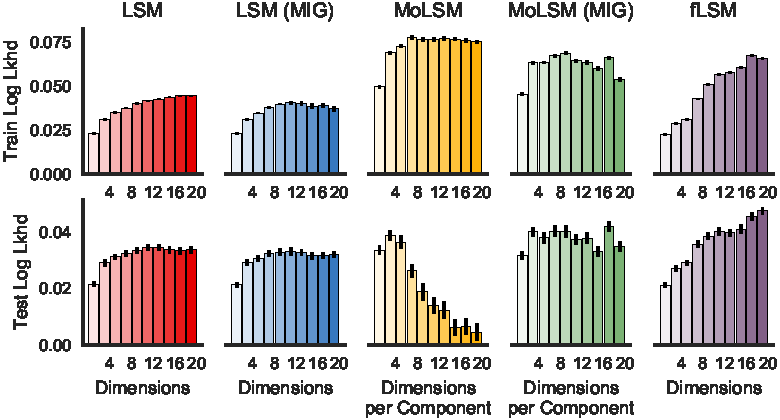
\includegraphics[width=\linewidth]{figures/lls.pdf}
\caption{\textit{Train and test likelihood for various
    latent space models (LSM) on brain network data as a function of
    latent dimensionality. Without a sparsity-inducing MIG prior,
    the mixture of LSMs (MoLSM) tends to over-fit the data, and with a prior its
    performance is comparable to the LSM.  The factorial LSM (fLSM)
    achieves high test performance by sharing embeddings across the
    entire population while letting individual networks use only a subset
    of the dimensions. Error bars denote~$\pm 1$ standard deviation.}}
\label{fig:lls}
\end{figure}


We compared the performance of the standard latent space model (LSM),
the mixture of latent space models (MoLSM), and the proposed factorial
generalization (fLSM). We studied the same brain connectivity
data as~\citet{durante2016nonparametric}. This dataset
contains ${N=42}$ networks, each with~${V=68}$ vertices.  We held
out~$24062$ randomly chosen edges for testing---approximately~$25\%$ of the
${\tfrac{1}{2}NV(V-1) = 95676}$ total number of edges---and trained
the models on the remaining edges. A simple independent Bernoulli model
(i.e.~${A_{n,[u,v]} \sim \distBernoulli(p_{u,v})}$) achieves~$77.8\%$
accuracy on the training data and~$76.5\%$ accuracy on the test data,
indicating that the networks are fairly stereotyped.

We measured performance as a function of number of latent dimensions,
which we varied from~$K=2$ to~$K=20$.  For the MoLSM, we fixed the
number of mixture components to~${H=10}$ and we varied the number of
dimensions per component from~$D=2$ to~$D=20$.  Thus, the MoLSM has
effectively ten times as many dimensions at its disposal, but
any given network may still only use~$D$ latent factors. Finally, we also
studied the effect of the multiplicative inverse gamma (MIG) prior for the
LSM and the MoLSM. (As argued above, the fLSM already benefits from a
sparsity inducing prior on the number of components used by any
network.)

We assessed the convergence of the Gibbs sampler by visually inspecting
the likelihood of the training data. We found that the samplers converged 
in less than~$100$ iterations for all models. Thus, we fit each model
with~$500$ iterations of Gibbs sampling, and computed training and test
likelihood 
estimates by averaging over the last~$250$ iterations.
For
each sample of the latent variables and parameters ($\bZ$,
$\{\widetilde{\bx}_b\}_{v=1}^V$, etc.), we computed the log
likelihood~\eqref{eq:flsm_lkhd} for both the training and test
data, subtracted the corresponding log likelihood under an independent
Bernoulli model, and normalized by the number of entries in the training
and test data, respectively. 
The MIG hyperparameters were set to~$a_1=3.5$ and~$a_2=2.5$, and the
mixture models were initialized with k-means clustering, as in~\citet{durante2016nonparametric}. The fLSM
hyperparameter was set to~${\alpha = \tfrac{K}{2}+1}$, such that the
prior probability of each feature is about~$\tfrac{1}{3}$ in expectation.

Figure~\ref{fig:lls} shows the log likelihoods of the training and
test data relative to the Bernoulli baseline. The standard LSM shows continued
improvement in training log likelihood as the number of dimensions
increases (red), though the test likelihood plateaus after about 10
dimensions. Incorporating an MIG prior biases the model toward using
fewer components, and we see that this additional regularization is
unnecessary for the standard LSM on this dataset (blue).  By contrast,
the mixture model shows severe over-fitting in the absence of
regularization (yellow).  Recall that here we are varying the number
of dimensions per component, and there are ten components total.  Some
mixture components only have two to five networks assigned to them,
which is insufficient to accurately infer the embedding.  With an MIG
prior, the MoLSM no longer exhibits this over-fitting, but the test
likelihoods are only comparable to that of the standard LSM.  Finally,
the fLSM seems to strike a nice balance.  By allowing factors to be
``turned off'' in some networks, it allows network-to-network
variability while forcing parameter sharing across the
population. This results in the highest performance: the baseline
performance is~$76.5\%$ accuracy on test data, and a 0.05 nat
improvement yields~$80.5\%$ accuracy.


\begin{figure}[t]
  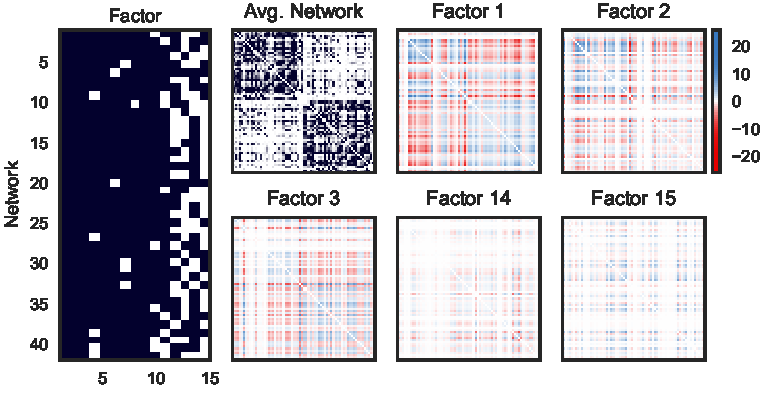
\includegraphics[width=\linewidth]{figures/factors.pdf}
  \vspace{-.4in}
  \caption{\textit{Inferred factors of the LSM and their usage. Left:
      a sample from the posterior distribution of factor
      usage. The~$n$-th row corresponds to the binary
      vector~$\widetilde{\bbm}_n$, where black denotes one and white
      denotes zero. Top: the average
      network~${\tfrac{1}{N}\sum_n \bA_n}$ exhibits strong block
      structure reflecting within-hemisphere connectivity.  Right:
      individual contributions of a subset of factors, as given
      by~$\bar{x}_k \bar{x}_k^\trans$.  Blue denotes increased
      probability of connection; red denotes decreased. Under the
      fLSM, each network~$n$ sums a subset of these factors. }}
\label{fig:factors}
\end{figure}

Figure~\ref{fig:factors} looks into the inferred factors of the fLSM.
The left panel shows a sample from the posterior distribution of factor
usage (i.e. a sample of~$\{\widetilde{\bbm}_n\}_{n=1}^N$). The factors
are sorted in decreasing order of magnitude~$\|\bar{\bx}_k\|_2$,
where~${\bar{\bx}_k = \left[ \widetilde{x}_{1,k}, \ldots, \widetilde{x}_{V,k} \right]}$.
We see that the first twelve factors are employed by almost all networks,
but the latter factors are more variable.  Of course, they are also
lower magnitude, and hence have a lesser impact on the resulting edge
probabilities.  This variability likely reflects both heterogeneity
in the population and posterior uncertainty.

The right panels of Figure~\ref{fig:factors} show the average network
(similar to Figure~9 of~\citet{durante2016nonparametric}) and then the
contributions of a few of the individual factors, i.e.~${\bar{\bx}_k \bar{\bx}_k^\trans}$.
Intuitively, the fLSM models the log-odds of a binary adjacency matrix
by summing a subset of these contributions.  We have not attempted to
read into these factors, but note how the strong
block structure emerges from the sum of individual factors.  One
next step would be to compare factor usage to other covariates of the
patients.  We expect that differences in network connectivity
arising from the features of an individual patient (age, disease history,
etc.) would be reflected in differences in factor usage as well.

\section{Conclusion}
\citet{durante2016nonparametric} present a mixture of latent space
models for capturing low-dimensional structure in populations of
networks.  Mixing over latent embeddings handles network-to-network
variability within the population and provides promising results
compared to other hierarchical models that assume a single set of
edge probabilities across all networks.  Their Bayesian
nonparametric approach allows flexible inference of the number of
mixture components and latent dimensions in a data-driven manner.

We present a generalization from the mixture
model to a factorial model in which the population of
networks share a set of latent factors, but only a subset of those
factors actively determine edge probabilities for any given network.
For example, in studying brain connectivity, the factorial model postulates
that a set of latent features determines the probability of fiber
tracts between two brain regions (e.g. age, diseases, drug use), and
each patient may possess a different subset of these features. By contrast,
the mixture model postulates a collection of different ``types'' of
patients, each with characteristic patterns of connectivity.
These two models are similar, but they may yield different
insights into the population of networks under study.

This suggests a number of avenues for future work.  In many cases, the
network itself is not directly observable; rather, we have
access to only indirect measurements, like neural spike trains, which
provide statistical information about the presence or absence of an
edge between two vertices.  In these cases, we would like to
perform joint inference of the network \emph{and} its underlying
structure, as in \citet{linderman2014discovering}
and~\citet{linderman2016bayesian}.  In other experiments, like
longitudinal studies of brain connectivity, the observed networks are
not exchangeable draws from a latent mixture or factor model, but
rather a sequence of observations that we expect to be correlated over
time, as in other dynamic network
models~\citep[e.g.][]{bassett2011dynamic, linderman2014framework}.
Likewise, while~\citet{durante2016nonparametric} mix
over complete network models, a natural alternative is to mix over
per-edge probabilities, as in the mixed-membership stochastic block
model~\citep{airoldi2008mixed}. In such models, each vertex pair
has an associated pair of latent discrete ``roles'', and the probability
of connection is a function of these underlying roles.  
Finally, as the authors mention, scaling inference to larger networks
is another area for future work. Variational inference
algorithms could be well suited to this challenge~\citep{jordan1999introduction, blei2017variational}. 


\bibliographystyle{apa}
\bibliography{refs.bib}

\end{document}






































